\section{The Pelican, the Poet, and the Puer}


\begin{quotex}
The union of the mathematician with the poet, fervor with measure, passion with correctness, this surely is the ideal.
\flright{\textsc{William James}}
\end{quotex}


\paragraph{Puer}


\begin{wrapfigure}{rt}{.3\textwidth}
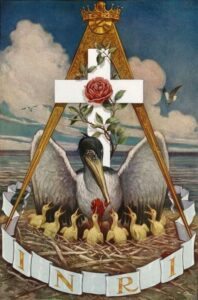
\includegraphics[width=.3\textwidth]{MotherPelican-198x300.jpg}
\end{wrapfigure}

There is great pleasure in being a boy. Everything is taken care of: food, shelter, travel, and so on. It leaves a boy with ample time to wonder about things. I used to wonder how the universe could possibly exist. The thought of such a huge and complex universe baffled me, the more I tried to imagine or conceive it. On the other hand, it was inconceivable for there to be nothing, so there had to be something.

I remember playing on the kitchen floor; there was one small window above the sink. In the morning, I would watch the rays of light streaming through it and then onto the floor. The beam of light reflecting in the dust fascinated me, since I could see it from the window to the floor.

My life seemed to be the most important. My family were archetypes: Father, Mother, Sister, Grandma, etc. On many Sundays we visited Grandma and drove back in the dark. I would stare out the car window and wondered where the other cars were going. I barely grasped that there are other people with lives.

Still young, I anticipated some great philosophical and scientific problems: existentialism, optics, solipsism. And these are just a few of the meditations of a boy.

\paragraph{Mater}





Mother was the center. It was impossible to envision her as a real human being rather than a mythical figure. Only within the past few years have I been able to understand her plans for me. She had me do complex arithmetic problems even before school age. She would buy me plastic model kits, mostly jets, missiles and some automobiles. (Yes, boys were allowed to use airplane glue.) I was subscribed to various magazines including Science Digest. After shopping trips, she would bring me back a Tom Corbett science fiction group. Clearly, I was being groomed for STEM before it was a ``thing''.

The symbol of the pelican feeding her babies from her own blood is ancient, going back to pagan days. The Christians adapted it for obvious reasons and it appears in many churched.

It is a symbol of charity (Dante referred to Christ as ``our Pelican''). My mother's love was an enduring presence, so much so that it was inconceivable to experience life without it.

\paragraph{Theoria}


I saw a random Twitter comment from a fellow who was concerned that studying mathematics would negatively affect his poetic skills. Of course not. Maths begin in wonder and only later does it harden into syntactic manipulations.

Every month, google sends me a report about Internet searches that point to gornahoor. I am always surprised that \emph{Naïve Set Theory}\footnote{\url{https://www.gornahoor.net/library/Halmos_NaiveSetTheory.pdf}} by \textbf{Paul Halmos} gets the most clicks. Unlike a strictly formal set theory, ``naïve'' in this case means something more like intuition. In \emph{Covenant of the Heart}, \textbf{Valentin Tomberg} writes:

\begin{quotex}
Intuition is the faculty of knowledge that results from instinct that is illumined by reason. It is what brings two opposite poles in humans to a unity, or unites what is most deeply implanted in them, which works hidden in darkness in the depths of their beings, with the reflecting faculty of intelligence, which is most bright in human beings, lying uppermost within them.
\end{quotex}


I was always good at mathematics and never had to study. People would ask me to tutor them. But I was horrible at it because I can just ``see'' the answer and there is no way to explain that. In a similar way, Axioms are just ``seen'' or ``intuited'', but never proved. Here are some naïve examples:

Why is there something rather than nothing? The \textbf{Axiom of Identity} shows that something exists, namely the being that is identical to itself. But that can only refer to God whose essence is existence. We, in our human state, are subject to privations which is a lack of full being; our existence never fully encapsulates essence.

The \textbf{Axiom of Infinity} describes the Infinite, and our understanding brings us into the mind of God. There is a genuine thrill when contemplating the cardinality of the continuum!

The \textbf{Axiom of Choice} proves free will. Sets don't operate on their own, so someone needs to be able to choose from one set in order to create another.

Finally, the \textbf{Axiom of Pairing} shows that sets can be ``paired up'': if A and B both exist, then so does A+B exist. For each A, there is a special B waiting in expectation.

\paragraph{Lux}


People falsely believe that the truth is only found in the light. But daylight hides the truth. The Sun is not yellow and the Sky is not blue; they are optical illusions. Those living in perpetual daylight would never suspect that there are heavenly bodies like the Moon, Planets, and the Stars.

Truth is hidden in the darkness. Nicodemus was initiated at night. But there are two kinds of darkness\footnote{\url{https://www.gornahoor.net/?p=15803}}. First there is the darkness of chaos, in which we cannot make out any distinct items.

The second is the night of the hidden revelation. It is God's truth that is hidden from the world. However, once God's truth is revealed, there is an inversion of all values. Then revelation is the light, and the world is embedded in darkness.


\flrightit{Posted on 2022-03-24 by Cologero}

\begin{center}* * *\end{center}

\begin{footnotesize}
\begin{sffamily}
\texttt{Tiffany Dawn Smith on 2022-03-25 at 18:22 said:}

Fascinating. Thank you.

\end{sffamily}
\end{footnotesize}

